% TEMPLATE for Usenix papers, specifically to meet requirements of
%  USENIX '05
% originally a template for producing IEEE-format articles using LaTeX.
%   written by Matthew Ward, CS Department, Worcester Polytechnic Institute.
% adapted by David Beazley for his excellent SWIG paper in Proceedings,
%   Tcl 96
% turned into a smartass generic template by De Clarke, with thanks to
%   both the above pioneers
% use at your own risk.  Complaints to /dev/null.
% make it two column with no page numbering, default is 10 point

% Munged by Fred Douglis <douglis@research.att.com> 10/97 to separate
% the .sty file from the LaTeX source template, so that people can
% more easily include the .sty file into an existing document.  Also
% changed to more closely follow the style guidelines as represented
% by the Word sample file. 

% Note that since 2010, USENIX does not require endnotes. If you want
% foot of page notes, don't include the endnotes package in the 
% usepackage command, below.

% This version uses the latex2e styles, not the very ancient 2.09 stuff.
\documentclass[letterpaper,twocolumn,10pt]{article}
\usepackage{usenix,epsfig,endnotes,placeins}
\begin{document}

%don't want date printed
\date{}

%make title bold and 14 pt font (Latex default is non-bold, 16 pt)
\title{\Large \bf SSID's and Social Networks}

%for single author (just remove % characters)
\author{
{\rm Michael Ballantyne}\\
University of Utah
\and
{\rm Maria Jenkins}\\
University of Utah
% copy the following lines to add more authors
\and
{\rm Priyanka Parekh}\\
University of Utah
} 

\maketitle

% Use the following at camera-ready time to suppress page numbers.
% Comment it out when you first submit the paper for review.
\thispagestyle{empty}


\subsection*{Abstract}
Some Wi-Fi network clients transmit a list of networks they've
previously connected to when scanning for networks to join, and many
users are not aware that this data is broadcasted and can be easily
monitored. We hope to make users aware that this data can reveal
information about locations they spend time and their social
connections. We captured Wi-Fi probe requests from a sample of
wireless clients and analyzed the social network implied in the data
for privacy risks. We found that Apple laptops revealed the most,
while most mobile devices and computers running Linux no longer share
private data in probe requests. The data suggests that while some
computers no longer reveal previous network associations, large scale
data from the remaining clients could present a significant privacy
risk. Even at small scale the list of network associations is a
possible tool for Wi-Fi client fingerprinting. Our work concurs with
other recent studies showing that network associations can be used to
fingerprint Wi-Fi clients or link users to certain political organizations or other groups based on the names of the networks. To encourage
users to be more security conscious we provided participants with a
personalized interactive social network graph showing how their
network associations relate them to other participants. We include
results from a survey conducted to understand participants' reactions
to this data.

\section{Introduction}
Laptops broadcast the list of Wi-Fi networks (SSID's) that a user has ever connected to. The list of SSID's is broadcasted when your laptop is attempting to connect to a Wi-Fi access point. Wi-Fi access points are ubiquitous and passive Wi-Fi tracking has started to become yet another way for retailers, advertisers, and data analytics companies to glean useful information about people. A quick google search for passive Wi-Fi tracking reveals tutorial after tutorial on passive Wi-Fi tracking. Previously cell phones broadcasted this data however recently they have stopped. A large majority of users are unaware that this metadata is being publicly broadcast and can be easily collected. The fact that this data is being broadcasted raises privacy and security concerns. From your SSID list it could be inferred what your favorite coffees shop is, your social and political affiliations and where you work among other things. It also raises some security concerns. An attacker could conduct a man-in-the-middle attack, an evil twin attack or Auto Association Karma Attack [Reference]. 

\section{Background}
Every wireless enabled device has to go through a discovery process to connect to a Wi-Fi access point. Devices can use passive or active scanning. There are three types of scans a device can deploy. There is a directed probe request where the client sends the list of SSID's to the access point in plain text. There is a broadcast probe where the client sends the MAC address of the device and asks for information on all the networks. There is a passive scan where the client waits for beacon frames. Beacon frames are packets that are broadcasted by the Wi-Fi access point and the device waits for a frame from an access point it has previously connected to. 

Different laptops use different probe request methods. Cell phones use a mixture of broadcast probes and passive scanning. To gather this data is trivial with access to a computer or Wi-Fi device. The laptop or Wi-Fi device can be put into monitor to pickup nearby traffic. In doing so the device in monitor mode is not broadcasting its presence, making it hard to detect if a nearby user is collected your metadata.

\section{Related Work}
There has been a fair amount of related work in this area, however most of the work was targeted at cell phones and not laptops. Cell phones have stopped broadcasting the SSID list when probing for Wi-Fi connections.

Chang et al  sought to discover user relationships from observing the similarity of SSID lists between users, they took into account physical proximity and spatio-temporal behavior. They looked at the similarities of SSID lists being broadcasted from cell phones before cell phones disabled this feature. They found that spatio-temporal data had more social connections. 

Barbera et al  used social network analysis on datasets of Wi-Fi probes from cell phones in public areas. They found that data matched typical properties of social networks. They also mentioned what devices broadcast the SSID list when probing for a connection.

Desmond et al discussed an alternative approach to fingerprinting that defeats MAC address 
randomization and the absence of an SSID list by timing the intervals between Wi-Fi probes, but requires hours of continuous data to perform adequately.

Cunche et al  present a mechanism to detect links between people by fingerprinting devices by exploiting the fact the SSID lists are broadcasted in plain text when probing for WI-FI connections. They take a very quantitative approach and are able to gather a large dataset. This work demonstrates a privacy breach allowed by the 802.11 probe requests and raises awareness that initiative should be taken to increase privacy in terms of Access point discovery. 

Greenstein et al makes the argument that it is in the best interest of not only users, but also manufacturers, to address the privacy threats that wireless networks pose. The authors considered an 802.11 case study and analyzed 802.11 traces. They used this information to show that, over time, devices can be identified and tracked through its SSID lists, its persistent link-layer address, and other characteristics. The authors of this work provide suggestions for ways to improve privacy through design considerations.

\section{Privacy Considerations}
To conduct this study we had to take into consideration the security and privacy of our participants so as to minimize harm but still collect meaningful data. We took precautionary measures to protect the anonymity of our users and the data we collected from them. 
All participants in the study were required to sign an informed consent. The informed consent notified the participants what data we would be collecting, how we would use it, and what our retention policies were. 
Participants who had SSID's that less than two other participants connected to were filtered out of the data. We assumed that most home networks would be filtered out this way and we would be left with general networks like coffee shops and campus wifi. We encrypted the data in transit and at rest in an effort to keep our users data anonymous and secure.


\section{Data Collection}


\section{Data Evaluation}
We were less successful in capturing data than we anticipated. Of our 28 participants (including the authors), 18 only yielded zero or one network name. Figure~\ref{histogram} shows the full distribution of network counts. Following data collection, we performed some further experiments to explain these disappointing results.

\begin{figure}
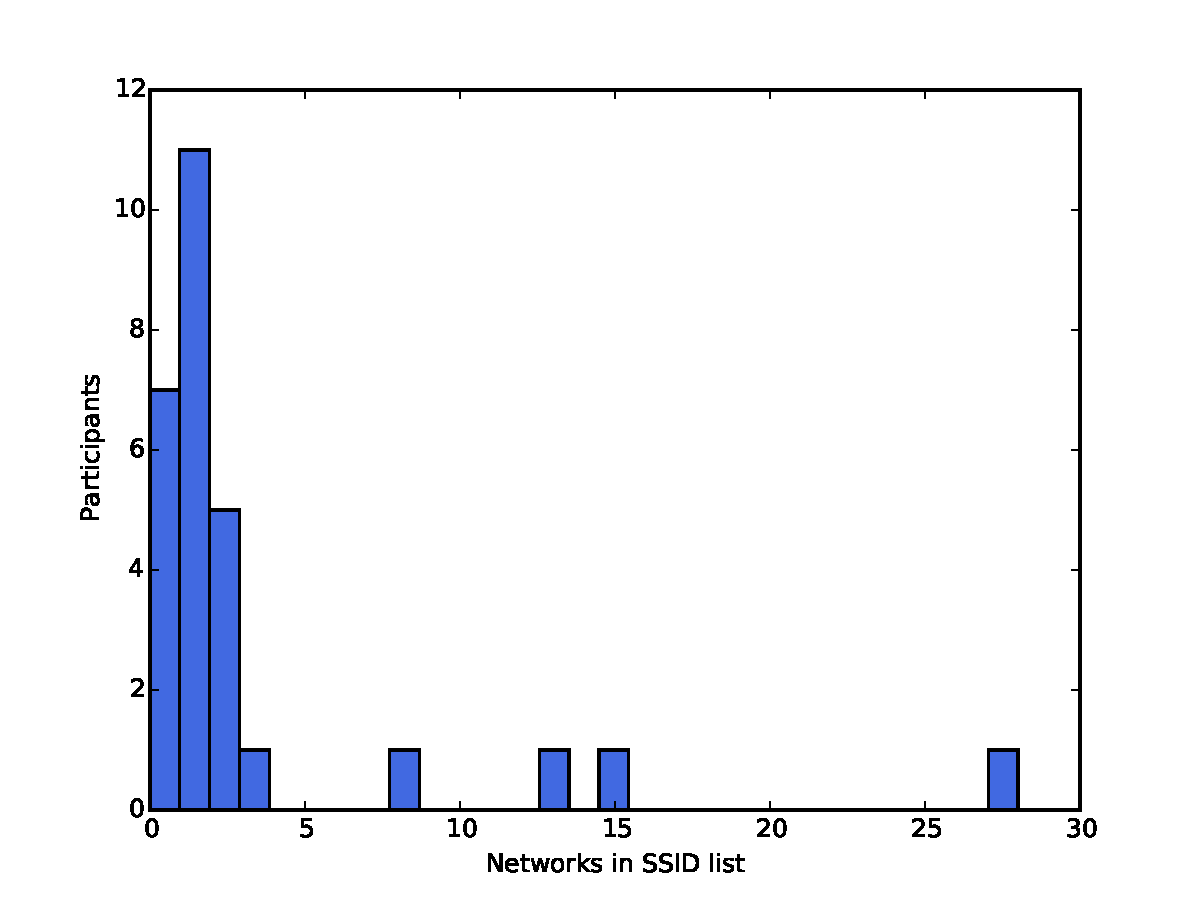
\includegraphics[width=\columnwidth]{hist.pdf}
\caption{Histogram of SSID list size}
\label{histogram}
\end{figure}

\FloatBarrier

\subsection{Capture Reliability}
The three individuals yielding the most network names were the authors. We hypothesize that more complete network lists were collected from our devices because they were present near the monitoring device for an extended period of time, so there were multiple opportunities to capture the data. As a test we measured the number of network names cumulatively collected by packet capture while a MacBook scanned for wireless networks a number of times. We found that a capture of only a single scan yielded on average only 31\% of the network list (with 28 networks total) and that we'd need to capture four or five scans to get a mostly-complete list. Figure~\ref{scans} shows the complete results of this experiment. An attacker able to monitor traffic over a long period of time likely wouldn't find this to be a problem, but it might thwart reliable fingerprinting of clients an access point only sees once. However, we suspect that our failure to capture the SSID list reliably was not because they were not transmitted, but because our receiver was overwhelmed and unable to keep up with filtering.

\subsection{Linux Socket Filtering}
During packet capture with scapy we found that the Wi-Fi Pineapple occasionally froze, requiring a restart, and at other times took several seconds to register new packets. We suspect that our packet filtering code in python wasn't able to keep up with the volume of captured packets. The Pineapple only has a 400 MHz processor, and each packet received must be communicated from kernel-space to user-space by a system call before it is filtered in python. Sometime after the data collection phase of our project we learned about linux socket filtering, a way to filter packets in kernel-space before they are returned to a packet monitoring application. Filters from tools like tcpdump typically use this method. The filtering rules available through tcpdump are sufficient to express the filter we'd written in scapy. Testing with tcpdump filtering shows that it reliably collects at least 16 of 28 networks from a single scan. It isn't clear why only 16 of the network names appear to be transmitted during a scan. Perhaps the laptop successfully established a connection before needing to complete the scan; more seem to be transmitted when initially enabling wireless in a location where none of the remembered wireless networks are available. Overall we suspect that if we'd used kernel level filtering during the data collection phase of our study we would have collected more network names from some of our participants.

\subsection{Operating System Behavior}
Another factor limiting the volume of data we captured was encouraging --- it appears that Linux and Windows clients don't generally perform directed probes, opting instead for broadcast probes unless a network was specially configured. During data collection we noted that captures from devices running Linux usually only included a single SSID plus a broadcast probe. The final social network graph discussed in section~\ref{social} shows many devices only having connected to UConnect, the campus wireless network. We hypothesize that Linux devices transmit directed probes only for the network they're currently connected to or were most recently connected to. Other networks are discovered by broadcast probes. Documentation for wpa\_supplicant on linux suggests that users could configure individual networks for which directed probes should be used, like hidden networks, but that otherwise it would use broadcast probes. We haven't found documentation for the behavior on Windows but we suspect that it similarly only uses directed probes for manually configured networks that may be hidden. Of the 5 devices in our study that yielded 3 or more network names, all were Apple devices. At least one of those devices was running the latest release of OS X, Yosemite.

These results suggest that vendors other than Apple have recognized the security and privacy implications of directed probes and modified their devices to instead use broadcast probes. Our testing suggests that Apple has done the same for its mobile devices, but not for OS X. Given that other platforms have demonstrated that broadcast probing works effectively we argue that Apple should change the behavior of OS X to better preserve privacy.

\begin{figure}
\centering
\begin{tabular}{l | l}
Scans & SSIDs Collected \\ 
\hline
1 & 31\% \\
2 & 53\% \\
3 & 63\% \\
4 & 89\% \\
5 & 91\% \\
\end{tabular}
\caption{SSID collection by number of network scans captured. Full SSID list is 29 networks. Averaged over 3 trials.}
\end{figure}
\begin{figure*}
\centering
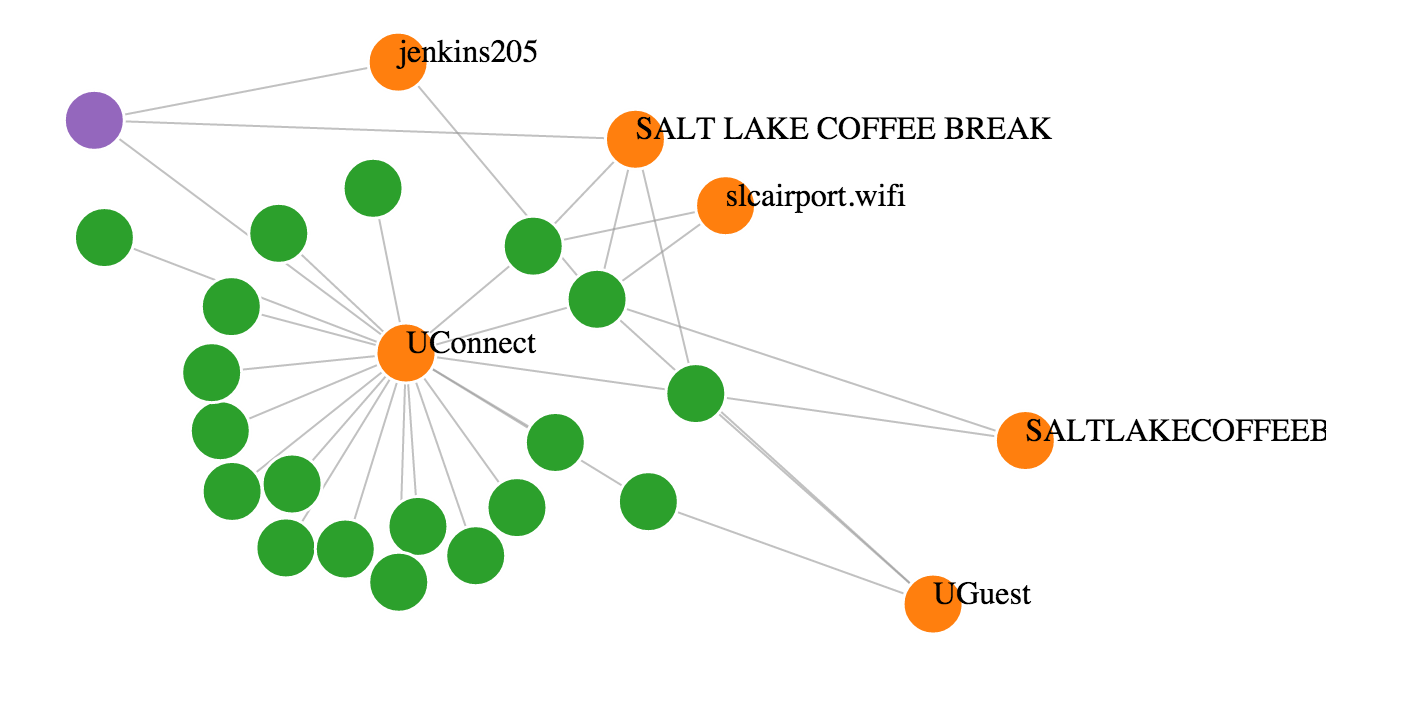
\includegraphics[scale=.5]{graph.png}
\caption{\textsf{Social network graph}}
\end{figure*}

\section{Social Network Analysis}
SSID lists and MAC addresses can be used to infer social networks and ties[CHANG ETAL]. Although we didn't gather enough data to infer large social networks we gathered enough to construct a graph of the participants and the SSID's the participants had in common. The filtered metadata was used to create personalized social network graphs for each participant. The graphs were rendered using Javascripts D3 library. The graphs were rendered and sent out to participants with an automated script so that their SSID lists and graphs were never looked at. 

Figure 3 is an example social network graph. The green nodes denote the anonmyized participants, the purple node indicates the participant, and the orange nodes denote the SSID's shared among participants. Along with the graph the list of SSID's that was broadcasted by the participants laptop was included. They are not pictured here to protect this individuals privacy. Wi-Fi access points were only included if more than two users had connected to them. We promised not to include the home network names and only one home network name had at least two particpants that had connected to it. It happened to be one of the authors home networks so received authorization to included it in the network graph. 

\section{Participant Survey}
We asked our participants to complete a survey after viewing their personalized social network graph.


\section{Future Work}

\section{Conclusion}







\end{document}